
\documentclass[tikz, border=1mm]{standalone}

\usepackage{amsmath}
\usepackage{tikz}

\usetikzlibrary{calc,angles,quotes}

\begin{document}
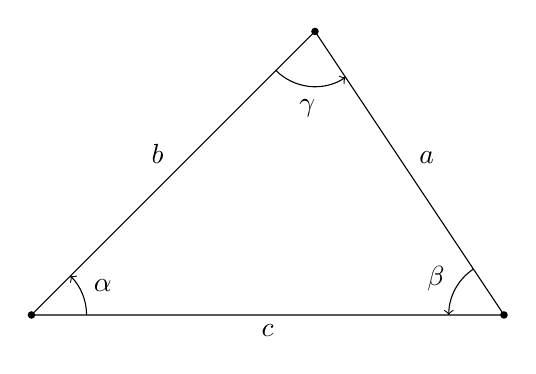
\begin{tikzpicture}[scale=1.2]

	\coordinate (A) at (0,0);
	\coordinate (C) at (5,0);
	\coordinate (B) at (3,3);

	\draw (A) -- (B) -- (C) -- cycle;

	\fill (A) circle (0.4mm);
	\fill (B) circle (0.4mm);
	\fill (C) circle (0.4mm);

	\node[above right] at ($(B)!0.5!(C)$) {$a$};
	\node[above left]  at ($(A)!0.5!(B)$) {$b$};
	\node[below] at ($(A)!0.5!(C)$) {$c$};

	\pic[draw, ->, "$\alpha$", angle radius=0.7cm, angle eccentricity=1.4]
	{angle = C--A--B};

	\pic[draw, ->, "$\beta$", angle radius=0.7cm, angle eccentricity=1.4]
	{angle = B--C--A};

	\pic[draw, ->, "$\gamma$", angle radius=0.7cm, angle eccentricity=1.4]
	{angle = A--B--C};

\end{tikzpicture}
\end{document}
